\documentclass{article}
\usepackage{graphicx} 
\usepackage[colorlinks=true, linkcolor=blue, urlcolor=red]{hyperref}
\usepackage[utf8]{inputenc}
\usepackage[T1]{fontenc}
\usepackage{lmodern} 
\usepackage[polish]{babel}
\usepackage{float} 
\usepackage{listings}
\usepackage{xcolor}

\lstnewenvironment{Rcode}[1][]{
    \lstset{
        language=R,
        basicstyle=\ttfamily,
        keywordstyle=\color{blue},
        commentstyle=\color{green!40!black},
        stringstyle=\color{orange},
        showstringspaces=false,
        frame=single,
        numbers=left,
        numberstyle=\tiny,
        numbersep=5pt,
        breaklines=true,
        #1
    }
}{}

\title{Statystyka Wielowymiarowa}
\author{Adam Staniszewski}
\date{May 2024}

\begin{document}

\maketitle

\tableofcontents  % Add table of contents here

\section{Dobór zbioru danych}
Do wykonywania zadań został wybrany zbiór \href{https://www.kaggle.com/datasets/girumwondemagegn/dataset-for-renewable-energy-systems}{Dataset for renewable energy systems}. Składa się on z 13 kolumn i około 15000 wierszy. 

Dodatkowo, dla zadań klasyfikacji binarnej, kolumna \textbf{Type\_of\_Renewable\_Energy} została przerobiona na 7 osobnych kolumn, reprezentujących źródła energii:
\begin{itemize}
    \item \textbf{Solar},
    \item \textbf{Wind},
    \item \textbf{Hydroelectric},
    \item \textbf{Geothermal},
    \item \textbf{Biomass},
    \item \textbf{Tidal},
    \item \textbf{Wave},
\end{itemize}

\section{Laboratorium 1}
\subsection{Regresja liniowa}
Na początku przeprowadzamy prostą regresję liniową:

\begin{figure}[H]
    \centering
    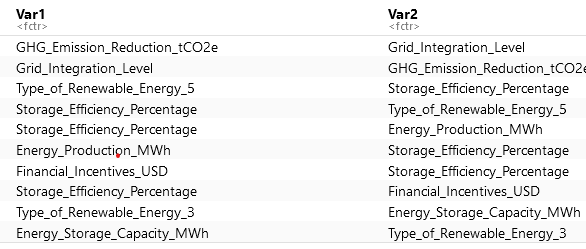
\includegraphics[width=0.9\linewidth]{obraz.png}
    \caption{Zmienna objaśniana - Installed Capacity MW. Zmienna objaśniająca - Energy Production MWh}
    \label{fig:regression}
\end{figure}

\begin{figure}[H]
    \centering
    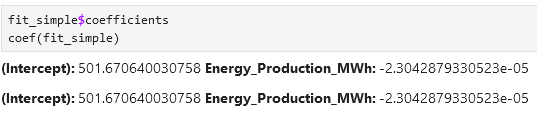
\includegraphics[width=0.9\linewidth]{obraz2.png}
    \caption{Współczynniki regresji}
    \label{fig:coefficients}
\end{figure}

\begin{figure}[H]
    \centering
    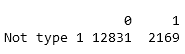
\includegraphics[width=0.9\linewidth]{obraz3.png}
    \caption{Podsumowanie regresji liniowej}
    \label{fig:summary}
\end{figure}

\begin{figure}[H]
    \centering
    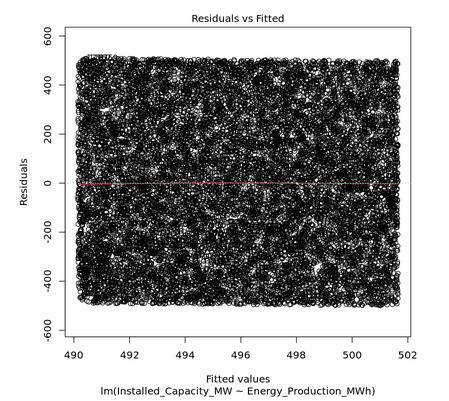
\includegraphics[width=0.9\linewidth]{obraz4.png}
    \caption{Wartości rzeczywiste vs przewidywane}
    \label{fig:real_vs_predicted}
\end{figure}

\begin{figure}[H]
    \centering
    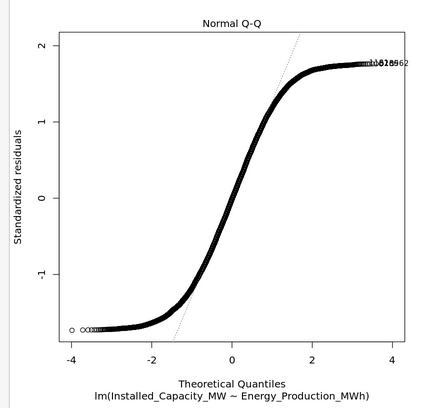
\includegraphics[width=0.9\linewidth]{obraz5.png}
    \caption{Reszty regresji}
    \label{fig:residuals}
\end{figure}

\begin{figure}[H]
    \centering
    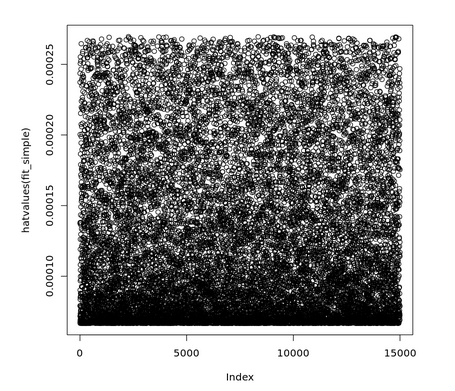
\includegraphics[width=0.9\linewidth]{obraz6.png}
    \caption{Heat values}
    \label{fig:heat_values}
\end{figure}

\subsection{Regresja wielokrotna}
Przejdźmy do regresji wielokrotnej. Będziemy przewidywać wartość \textbf{Installed\_Capacity\_MW} na podstawie zmiennych \textbf{Energy\_Production\_MWh} i \textbf{Energy\_Consumption\_MWh}.

\section{Laboratorium 2}
\subsection{One hot encoding}
\subsection{GLM}
\subsection{Podział zbioru}
\subsection{Metoda LDA}
\subsection{Metoda QDA}
\subsection{Metoda kNN}

\section{Laboratorium 3}
\subsection{Walidacja krzyżowa}
\subsubsection{Metoda zbioru walidacyjnego}
Na początku wczytuję dane, usuwam wartości NaN i przygotowuję zbiór walidacyjny.

\begin{Rcode}
energy_data <- read.csv("energy_dataset.csv")
energy_data <- na.omit(energy_data)
set.seed(1)
n <- nrow(energy_data)
train <- sample(n, n / 2)
\end{Rcode}
Dopasowuję model liniowy na zbiorze uczącym i obliczam MSE dla zbioru walidacyjnego:

\begin{Rcode}
energy_lm <- lm(Type_of_Renewable_Energy ~ Energy_Production_MWh,
                 data = energy_data,
                 subset = train)

validation_set <- energy_data[-train,]

mse <- mean((validation_set$Type_of_Renewable_Energy -
              predict(energy_lm, validation_set))^2)

\end{Rcode}
Otrzymana wartość MSE: \textbf{4.0439057662439}.

Użyjmy wielomianów o różnych stopniach:

\end{Rcode}
Dopasowuję model liniowy na zbiorze uczącym i obliczam MSE dla zbioru walidacyjnego:

\begin{Rcode}
for (i in 2:5) {
  energy_lm_poly <- lm(Type_of_Renewable_Energy ~ poly(Energy_Production_MWh, degree = i), data = energy_data, 
                     subset = train)
  print(mean((validation_set$Type_of_Renewable_Energy - predict(energy_lm_poly, validation_set))^2))
}
\end{Rcode}
Otrzymujemy MSE: 

\begin{Rcode}
[1] 4.042959
[1] 4.041494
[1] 4.041374
[1] 4.042979
\end{Rcode}
\textbf{Wniosek} - stopień wielomianu w tym przypadku nie ma znaczącego wpływu na otrzymany MSE.
Powtarzam obliczenia dla innego zbioru walidacyjnego:

\begin{Rcode}
degree_max <- 5

compute_mse <- function(degree, train) {
  energy_lm <- lm(Type_of_Renewable_Energy ~ poly(Energy_Production_MWh, degree), data = energy_data, subset = train)
  validation_set <- energy_data[-train,]
  mean((validation_set$Type_of_Renewable_Energy - predict(energy_lm, validation_set))^2)
}

mse <- vapply(1:degree_max, compute_mse, FUN.VALUE = numeric(1), train = train)
\end{Rcode}
Otrzymane wartości MSE:
\begin{Rcode}
4.04390576624393
4.04295881295649
4.04149420436449
4.04137383913034
4.04297885010734
\end{Rcode}

\begin{figure}[H]
    \centering
    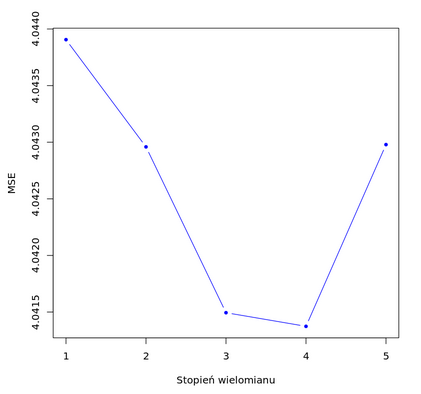
\includegraphics[width=0.8\linewidth]{obraz8.png}
    \caption{Zależność między wartością MSE a stopniem wielomianu.}
    \label{fig:enter-label}
\end{figure}

\subsubsection{Walidacja krzyżowa bez jednego (leave-one-out)}

\begin{Rcode}
compute_loocv_mse <- function(degree) {
  energy_glm <- glm(Type_of_Renewable_Energy ~ poly(Energy_Production_MWh, degree), data = energy_data)
  cv.glm(energy_data, energy_glm)$delta[1]
}
mse <- sapply(1:degree_max, compute_loocv_mse)
mse
\end{Rcode}

\begin{Rcode}
    TUTAJ WYKRES TEGO WYZEJ
\end{Rcode}

\begin{Rcode}
[Co teraz z wnioskami na temat regresji wielomianowej w naszym przypadku?]
[Sprawdź, że dla LOOCV obie współrzędne delta zawierają praktycznie to samo.]
\end{Rcode}

\subsubsection{K-krotna walidacja krzyżowa}
Tym razem jawnie ustawiamy parametr K oznaczający liczbę grup:

\begin{Rcode}
compute_kcv_mse <- function(degree, k) {
    energy_glm <- glm(Type_of_Renewable_Energy ~ poly(Energy_Production_MWh, degree), data = energy_data)
    cv.glm(energy_data, energy_glm, K = k)$delta[1]
}
mse <- sapply(1:degree_max, compute_kcv_mse, k = 10)
\end{Rcode}
Zestawiamy 10 wyników:
\begin{Rcode}
mse10 <- replicate(10, sapply(1:degree_max, compute_kcv_mse, k = 10))
\end{Rcode}
Otrzymujemy:
\begin{Rcode}
    10 WYNIKOW
\end{Rcode}
\begin{Rcode}
    WYKRES
\end{Rcode}
\begin{Rcode}
    CO Z WYNIKAMI
\end{Rcode}

\subsubsection{Bootstrap}
\begin{Rcode}

}
\end{Rcode}

\subsection{Selekcja cech dla modeli liniowych}
\subsubsection{Selekcja krokowa do przodu i wstecz}
\subsubsection{Wybór modelu przy pomocy metody zbioru walidacyjnego}
\subsubsection{Wybór modelu przy pomocy k-krotnej walidacji krzyżowej}

\end{document}
